\documentclass[10pt]{beamer} 
%设置为 Beamer 文档类型,设置字体为 10pt,长宽比为16:9,数学字体为 serif 风格
\usepackage[UTF8]{ctex}
\usepackage{float}
% Useful packages
\usepackage{braket}
\usepackage{color}
\usepackage{amsmath}
\usepackage{graphicx}
%Information to be included in the title page:
\title[About Beamer] %optional
{Electrodynamics Lecture 1-2}
\subtitle{mathmatical knowledge and skills}
\author % (optional, for multiple authors)
{Yuxuan Zhang }
\institute[VFU] % (optional)
{
  School of Physics \quad
  Zhejiang University
}

\date[VLC 2021] % (optional)
{May 4th 2023}

\begin{document}
\frame{\titlepage}

\begin{frame}
    \frametitle{目录}
    \tableofcontents
\end{frame}
\section{曲线坐标}
\begin{frame}
\frametitle{曲线坐标}
\begin{itemize}
    \item ($q_1,q_2,q_3$) $\rightarrow$ 一个三维空间中的点 $\quad$ 与直角坐标相互转换
    \item 等值面
    \item 坐标曲线 $\rightarrow$ 正交曲线坐标系
\end{itemize}
\end{frame}

\begin{frame}
    \frametitle{曲线坐标}
    \begin{itemize}
        \item 三个方向上微元弧的长度和方向\\
        $\vec{e_1},\vec{e_2},\vec{e_3}$用$\vec{i},\vec{j},\vec{k}$表示\\
        $|dl_1| = \sqrt{\left( \frac{\partial x}{\partial q_1}\right)^2+\left( \frac{\partial x}{\partial q_2}\right)^2+\left( \frac{\partial x}{\partial q_3}\right)^2}$

        \item $\vec{e_1} \rightarrow \frac{\partial \vec{r}}{\partial q_1}$\\
        反过来 $\vec{i} (\vec{e_1},\vec{e_2},\vec{e_3})$
        \item 应用:柱坐标系和球坐标系
    \end{itemize}
\end{frame}
\section{曲线坐标中的场微分}
\begin{frame}
    \frametitle{曲线坐标中的场微分}
    \begin{itemize}
        \item 梯度的表达式 (引出$\nabla $算子)
        \item $\nabla = \vec{e_1} \frac{1}{H_1}\frac{\partial}{\partial q_1}+\vec{e_1} \frac{1}{H_2}\frac{\partial}{\partial q_2}  +\vec{e_1} \frac{1}{H_3}\frac{\partial}{\partial q_3}$
        \item 散度和旋度的计算公式
        \begin{figure}
            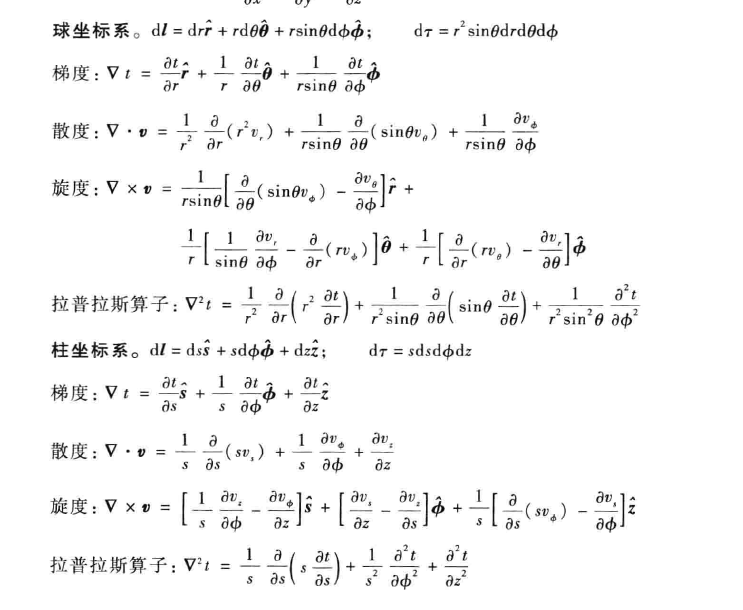
\includegraphics[scale = 0.4]{fig1.png}
        \end{figure}
    \end{itemize}
\end{frame}


\section{ $\nabla$ 符号与简单场论}
\begin{frame}
    \frametitle{ $\nabla$ 符号与简单场论}
    \begin{itemize}
        \item $\nabla \cdot (\nabla \times \vec{A}) \equiv 0$
        \item $\nabla \times (\nabla \phi) \equiv 0$
    \end{itemize}
\end{frame}

\section{积分微分回顾}
\begin{frame}
    \frametitle{ 积分计算回顾}
    \begin{itemize}
        \item 二重积分
        \item 三重积分
        \item 第一类曲线积分——线段元参数化为一定区间内的定积分
        \item 第一类曲面积分——曲面元参数化为一定区域的二重积分
        \item 第二类曲线积分——先化为第一类曲线积分
        \item 第二类曲面积分——先化为第一类曲面积分
    \end{itemize}
\end{frame}


\end{document}
